\documentclass[aspectratio=169,11pt]{beamer}

\usepackage{graphicx}
\usepackage{tikz}
\usetikzlibrary{positioning,arrows.meta}
\usepackage{xcolor}
\usepackage{booktabs}
\usepackage{tabularx}
\usepackage{array}
\usepackage{ragged2e}

\definecolor{GEUBlue}{RGB}{20,55,105}
\definecolor{GEULightBlue}{RGB}{238,244,251}
\definecolor{GEUGrey}{RGB}{90,90,90}
\definecolor{GEULightGrey}{RGB}{245,246,248}
\definecolor{RQRed}{RGB}{190,30,45}

\usetheme{default}
\setbeamertemplate{navigation symbols}{}
\setbeamertemplate{blocks}[rounded][shadow=false]
\setbeamercolor{normal text}{fg=black,bg=white}
\setbeamercolor{frametitle}{fg=GEUBlue}
\setbeamercolor{structure}{fg=GEUBlue}
\setbeamercolor{block title}{fg=GEUBlue,bg=GEULightBlue}
\setbeamercolor{block body}{fg=black,bg=GEULightBlue}
\setbeamerfont{frametitle}{size=\Large,series=\bfseries}

\newcommand{\GEULogo}{graphicera_logo.png}

\setbeamertemplate{headline}{%
  \begin{tikzpicture}[remember picture,overlay]
    \node[anchor=north east,xshift=-0.30cm,yshift=-0.12cm]
      at (current page.north east)
      {\includegraphics[height=0.62cm]{\GEULogo}};
  \end{tikzpicture}
  \vspace{0.72cm}
}
\setbeamertemplate{frametitle}{%
  \vspace{0.03cm}
  \insertframetitle\par
  \vspace{0.04cm}
  \textcolor{GEUBlue}{\rule{\textwidth}{0.9pt}}
  \vspace{0.03cm}
}
\setbeamertemplate{footline}{%
  \leavevmode
  \hbox{%
  \begin{beamercolorbox}[wd=.82\paperwidth,ht=0.32cm,dp=0.10cm,leftskip=.3cm]{author in head/foot}
    \tiny Department of Computer Science \& Engineering | Graphic Era (Deemed to be University)
  \end{beamercolorbox}%
  \begin{beamercolorbox}[wd=.18\paperwidth,ht=0.32cm,dp=0.10cm,rightskip=.3cm]{date in head/foot}
    \hfill\tiny\insertframenumber/\inserttotalframenumber
  \end{beamercolorbox}}
}

\newcommand{\smallnote}[1]{\vspace{0.08cm}{\scriptsize\color{GEUGrey}#1}}

\title{\textbf{Project-Based Learning}\\[2mm]\large Phase-I Evaluation}
\author{\textbf{RESQ}}
\institute{Department of Computer Science \& Engineering\\Graphic Era (Deemed to be University), Dehradun}
\date{Academic Session 2026--27}

\begin{document}

% 1 -- Title
\begin{frame}[plain]
\begin{tikzpicture}[remember picture,overlay]
\draw[GEUBlue,line width=3pt] (current page.north west) -- (current page.north east);
\node[anchor=north east,xshift=-0.45cm,yshift=-0.35cm] at (current page.north east)
{\includegraphics[height=1.0cm]{\GEULogo}};
\node[align=center,text width=.84\paperwidth] at ([yshift=.30cm]current page.center)
{{\color{GEUBlue}\fontsize{26}{30}\selectfont\bfseries PROJECT-BASED LEARNING}\\[3mm]
 {\fontsize{18}{22}\selectfont PHASE-I EVALUATION}\\[7mm]
 {\color{RQRed}\fontsize{22}{26}\selectfont\bfseries RESQ}\\[1.5mm]
 {\color{GEUGrey}\large\bfseries Intelligent Disaster Rescue \& Emergency Response Simulator}\\[2mm]
 {\color{GEUBlue}\normalsize\itshape ``Algorithms That Save Lives''}\\[4mm]
 {\color{GEUBlue}\small Team ID: DSCPP-III-2026-T117 \quad|\quad Mentor: Mr.\ Prabhdeep Singh}};
\node[align=center,anchor=south,yshift=.42cm] at (current page.south)
{\bfseries Department of Computer Science \& Engineering\\
Graphic Era (Deemed to be University), Dehradun\\[-1mm]
\scriptsize Academic Session 2026--27};
\end{tikzpicture}
\end{frame}

% 2 -- Team
\begin{frame}{Team \& Mentor Details}
\begin{columns}[T,totalwidth=\textwidth]
\column{.42\textwidth}
\begin{block}{Team Information}
\small
\begin{tabular}{@{}ll@{}}
\textbf{Team ID:} & DSCPP-III-2026-T117\\
\textbf{Semester:} & 3rd\\
\textbf{Sections:} & ML-1, ML-2, ML-4, DS-2\\
\textbf{Domain:} & Emergency Response\\
 & Systems (DSA + OOP)
\end{tabular}
\end{block}
\column{.56\textwidth}
\begin{block}{Team Members}
\scriptsize
\begin{tabularx}{\textwidth}{@{}p{0.4cm}Xp{1.85cm}@{}}
1. & \textbf{Vanya Rathi} (Team Leader) & 2510383410\\
2. & Akshat Dobhal & 2510370353\\
3. & Ayush Kandwal & 2510380235\\
4. & Nitin Singh & 2510370229
\end{tabularx}
\end{block}
\end{columns}
\vspace{2mm}
\begin{block}{Mentor}
Mr.\ Prabhdeep Singh
\hfill
\textbf{Interactions completed:} 02
\end{block}
\end{frame}

% 3 -- Problem & Motivation
\begin{frame}[shrink=12]{Problem Statement \& Motivation}
\begin{block}{Problem Statement}
\small In an earthquake, flood, fire or big road accident, a control room gets far more calls than the
teams, ambulances and beds it actually has free. The order of dispatch is decided by hand, mostly in the
order the calls came in, and the map app keeps sending units down roads that have already collapsed. So a
critical victim waits behind a stable one and the golden hour goes by. RESQ adds the layer that is missing
here: \textbf{who to rescue first, which unit to send, and which road is still open}.
\end{block}
\vspace{1mm}
\begin{columns}[T,totalwidth=\textwidth]
\column{.48\textwidth}
\textbf{\color{GEUBlue}Motivation}
\begin{itemize}\itemsep2pt
\small
\item An operator cannot re-rank hundreds of live calls by hand.
\item Map and CAD tools assume the roads are still intact.
\item A cut-off sector is usually found only after a unit gets stuck.
\end{itemize}
\column{.48\textwidth}
\textbf{\color{GEUBlue}Target Users / Stakeholders}
\begin{itemize}\itemsep2pt
\small
\item Control rooms (112 / 108 dispatchers).
\item NDRF / SDRF teams, ambulance crews, hospitals.
\item Students who want to see DSA used on a real problem.
\end{itemize}
\end{columns}
\end{frame}

% 4 -- Objectives & Proposed Solution
\begin{frame}[shrink=28]{Objectives \& Proposed Solution}
\begin{columns}[T,totalwidth=\textwidth]
\column{.48\textwidth}
\textbf{\color{GEUBlue}Project Objectives}
\begin{enumerate}\itemsep2pt
\small
\item Take in rescue calls and keep every victim record in a linked list.
\item Sort victims with a max-heap priority queue, using severity plus how long they have waited.
\item Keep the disaster area as a weighted graph and find the shortest route with Dijkstra.
\item Use BFS to spot isolated sectors, so cut-off victims can be sent to air support.
\item Put the whole simulation inside a C++ OOP engine and keep a stack as the audit trail.
\end{enumerate}
\vspace{1mm}
\textbf{\color{GEUBlue}Key Features}
\begin{itemize}\itemsep2pt
\small
\item Four scenarios: earthquake, flood, fire, highway pile-up.
\item Disaster-aware edge weights (epicentre slowdown, collapsed roads).
\item RED victims routed only to trauma-capable hospitals.
\item ``CUT OFF (BFS)'' flag for isolated sectors.
\end{itemize}
\column{.48\textwidth}
\textbf{\color{GEUBlue}Proposed Approach}
\begin{enumerate}\itemsep2pt
\small
\item \textbf{Input:} rescue call -- name, age, location, severity (RED/YELLOW/GREEN).
\item \textbf{Triage:} max-heap priority queue; FIFO queue for routine calls.
\item \textbf{Map:} weighted adjacency graph of the disaster area; blocked roads removed.
\item \textbf{Routing:} Dijkstra for unit\,$\rightarrow$\,victim\,$\rightarrow$\,hospital; BFS for reachability.
\item \textbf{Output:} route plan, ETA and a live operations dashboard.
\end{enumerate}
\vspace{1mm}
\begin{center}
\colorbox{GEULightBlue}{\parbox{.94\textwidth}{\centering\small
\textbf{Key Objective:} On the same scenario, reach RED (critical) victims faster on average than a
plain first-come-first-served dispatch does.}}
\end{center}
\end{columns}
\end{frame}

% 6 -- Course integration
\begin{frame}[shrink=10]{Integration of PBL Course Concepts}
\scriptsize
\begin{center}
\renewcommand{\arraystretch}{1.15}
\begin{tabularx}{.97\textwidth}{@{}>{\bfseries}p{2.7cm}X p{3.1cm}@{}}
\toprule
Course & Concepts Applied & Project Module\\
\midrule
Data Structures in C & Linked list (victim records), queue (routine calls),
max-heap priority queue (triage), stack (operation history) &
\texttt{linked\_list.c}, \texttt{queue.c}, \texttt{priority\_queue.c}, \texttt{stack.c}\\
Data Structures in C & Graph (disaster map), BFS (area exploration), Dijkstra (shortest route),
insertion \& quick sort, binary \& linear search &
\texttt{graph.c}, \texttt{sort\_search.c}\\
\midrule
OOPs with C++ & Classes \& objects (\textit{Victim, Location, Hospital, Disaster}),
encapsulation, constructors/destructors &
\texttt{resq.hpp}\\
OOPs with C++ & Inheritance \& polymorphism --- abstract \textit{RescueUnit} specialised
into \textit{RescueTeam} / \textit{Ambulance}; \textit{RescueOperation} engine &
\texttt{resq.cpp}, \texttt{main.cpp}\\
\bottomrule
\end{tabularx}
\end{center}
\vspace{1mm}
\begin{center}
\colorbox{GEULightBlue}{\parbox{.88\textwidth}{\centering
\textbf{Integration:} the C layer gives us the data structures and algorithms, and the C++ layer puts
them together into a single object-oriented simulation engine.}}
\end{center}
\end{frame}

% 7 -- Architecture
\begin{frame}{System Architecture / Workflow}
\begin{center}
\resizebox{\textwidth}{!}{%
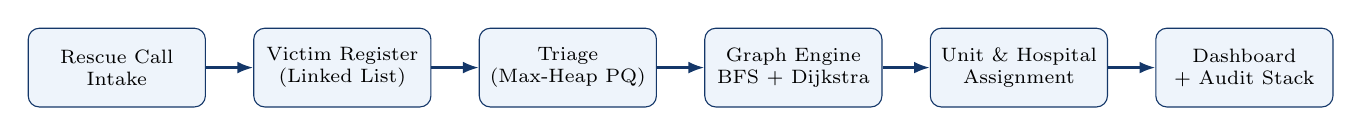
\begin{tikzpicture}[
node distance=6mm,
box/.style={rectangle,rounded corners,draw=GEUBlue,fill=GEULightBlue,
minimum width=2.25cm,minimum height=10mm,align=center,font=\scriptsize},
arrow/.style={-{Latex[length=2mm]},thick,draw=GEUBlue}
]
\node[box] (a) {Rescue Call\\Intake};
\node[box,right=of a] (b) {Victim Register\\(Linked List)};
\node[box,right=of b] (c) {Triage\\(Max-Heap PQ)};
\node[box,right=of c] (d) {Graph Engine\\BFS + Dijkstra};
\node[box,right=of d] (e) {Unit \& Hospital\\Assignment};
\node[box,right=of e] (f) {Dashboard\\+ Audit Stack};
\draw[arrow] (a)--(b); \draw[arrow] (b)--(c); \draw[arrow] (c)--(d);
\draw[arrow] (d)--(e); \draw[arrow] (e)--(f);
\end{tikzpicture}}
\end{center}
\vspace{3mm}
\begin{columns}[T,totalwidth=\textwidth]
\column{.48\textwidth}
\textbf{\color{GEUBlue}Major Components}
\begin{itemize}\itemsep2pt
\small
\item C DSA core --- list, queue, heap, stack, graph.
\item C++ OOP engine --- units, hospitals, disasters, operations.
\item Visual simulator --- map, queue view, dashboard.
\end{itemize}
\column{.48\textwidth}
\textbf{\color{GEUBlue}Data / Control Flow}
\begin{itemize}\itemsep2pt
\small
\item A call is saved, given a score and pushed into the heap.
\item The disaster changes the edge weights, or blocks edges completely.
\item Dijkstra returns the route, and the finished operation goes on the history stack.
\end{itemize}
\end{columns}
\end{frame}

% 8 -- Live demo
\begin{frame}{Live Demo --- Route Map \& Operations Dashboard}
\begin{columns}[T,totalwidth=\textwidth]
\column{.49\textwidth}
\begin{center}
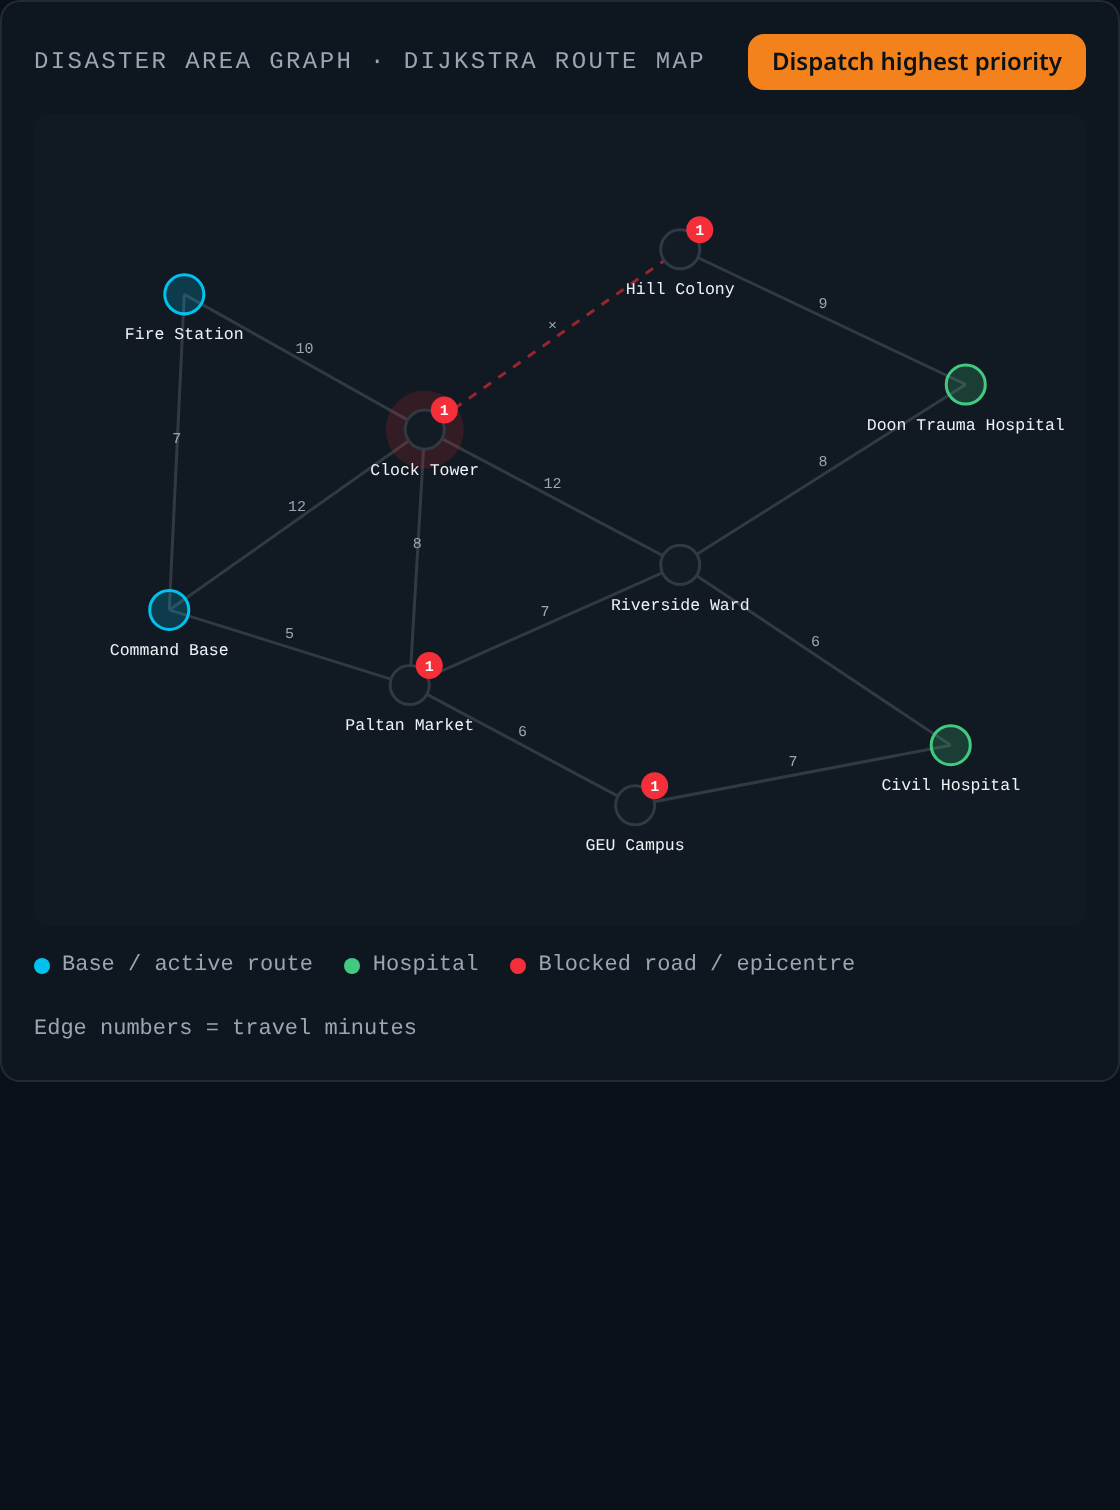
\includegraphics[width=\textwidth,height=.46\textheight,keepaspectratio]{demo1.png}
\end{center}
\vspace{1mm}
{\tiny\color{GEUGrey}\RaggedRight Max-heap re-orders the queue by severity; Dijkstra routes the unit to the victim and then to the hospital, around collapsed roads.\par}
\column{.49\textwidth}
\begin{center}
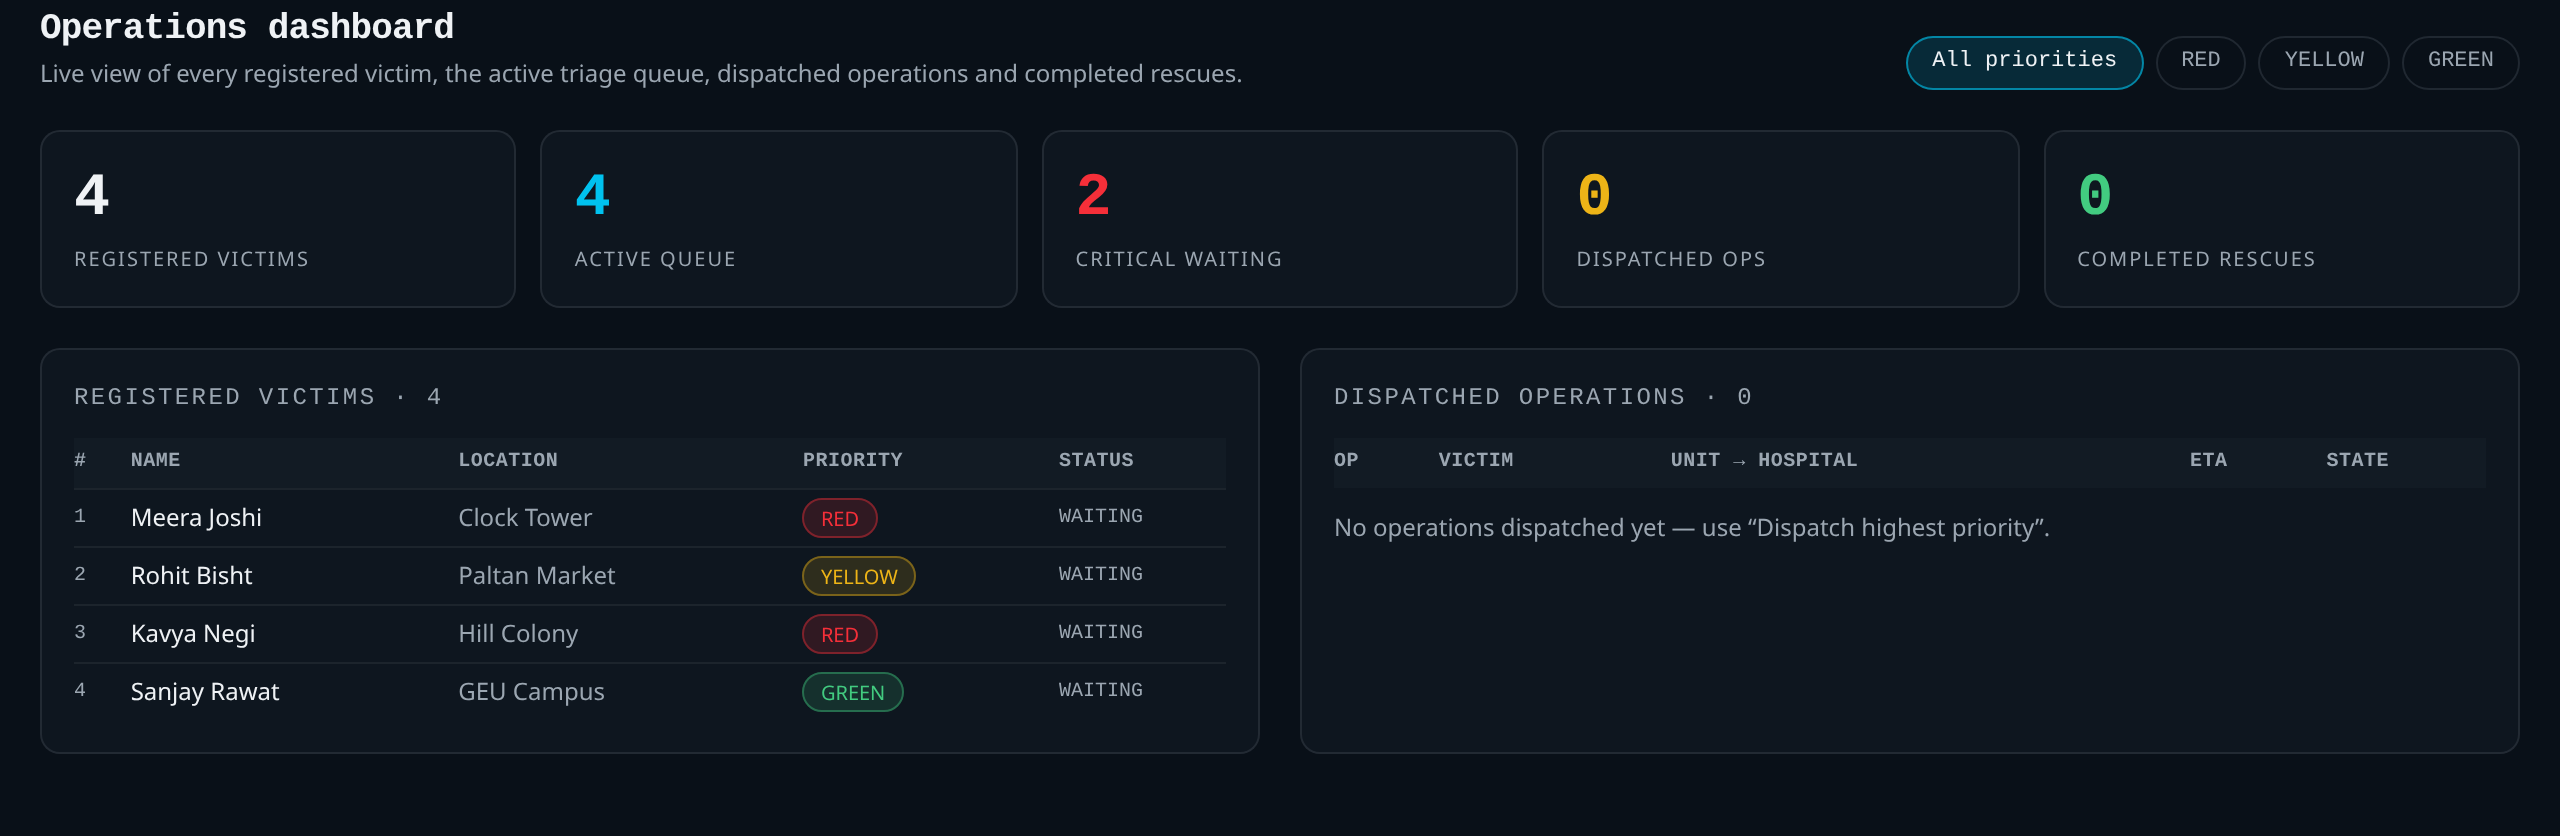
\includegraphics[width=\textwidth,height=.46\textheight,keepaspectratio]{demo2.png}
\end{center}
\vspace{1mm}
{\tiny\color{GEUGrey}\RaggedRight Dashboard: registered victims, active queue, critical victims waiting, dispatched operations and completed rescues, filterable by priority.\par}
\end{columns}
\end{frame}

% 9 -- Tech stack
\begin{frame}{Technology Stack \& Methodology}
\begin{columns}[T,totalwidth=\textwidth]
\column{.48\textwidth}
\begin{block}{Technology Stack}
\begin{itemize}\itemsep2pt
\small
\item Programming: C (C11) for DSA, C++ (C++17) for OOP
\item Build: GNU Make, \texttt{gcc}/\texttt{g++} with \texttt{-Wall -Wextra}
\item Visual demo: browser-based simulator mirroring the same algorithms
\item IDE: VS Code
\item Version Control: Git / GitHub
\end{itemize}
\end{block}
\column{.48\textwidth}
\begin{block}{Development Methodology}
\begin{enumerate}\itemsep2pt
\small
\item Requirement analysis of dispatch workflow
\item System design --- data structures \& class hierarchy
\item Incremental implementation, module by module
\item Testing on three disaster scenarios
\item Evaluation against FCFS baseline
\end{enumerate}
\end{block}
\end{columns}
\vfill
\begin{center}
\smallnote{We picked C because it gives direct control over memory and pointer-based structures, and C++ because
inheritance and polymorphism let us add a new type of rescue unit without touching the algorithms.}
\end{center}
\end{frame}

% 10 -- Progress & contribution
\begin{frame}{Initial Progress \& Team Contribution}
\begin{columns}[T,totalwidth=\textwidth]
\column{.42\textwidth}
\textbf{\color{GEUBlue}Progress Achieved}
\begin{itemize}\itemsep2pt
\small
\item Read up on triage protocols and how dispatch works
\item Fixed the requirements and the test scenarios
\item Drew the architecture and the class diagram
\item Wrote the C modules: list, queue, heap, stack and graph
\item Got the C++ engine and the visual demo running end to end
\end{itemize}
\column{.54\textwidth}
\textbf{\color{GEUBlue}Individual Contribution}
\vspace{1.5mm}
\scriptsize
\begin{tabularx}{\textwidth}{@{}p{2.0cm}p{1.9cm}X@{}}
\toprule
Member & Role & Contribution\\
\midrule
Vanya Rathi & Team Lead & Architecture, triage logic, integration, documentation\\
Akshat Dobhal & Developer & Linked list, queue, priority queue, stack\\
Ayush Kandwal & Developer & Graph module, BFS \& Dijkstra routing\\
Nitin Singh & Dev / Testing & C++ classes, scenario testing, dashboard \& reports\\
\bottomrule
\end{tabularx}
\end{columns}
\end{frame}

% 11 -- Roadmap & references
\begin{frame}[shrink=8]{Roadmap, Expected Outcomes \& References}
\begin{columns}[T,totalwidth=\textwidth]
\column{.47\textwidth}
\textbf{\color{GEUBlue}Roadmap}
\begin{enumerate}\itemsep2pt
\small
\item Phase-I: proposal, design, core DSA modules
\item Phase-II: C++ engine, multi-unit allocation
\item Phase-III: final simulator, comparison, demo
\end{enumerate}
\vspace{1.5mm}
\textbf{\color{GEUBlue}Expected Outcomes}
\begin{itemize}\itemsep2pt
\small
\item A working C/C++ simulator with a visual demo
\item Measured time saved for critical victims over FCFS
\item A log of every rescue operation that was carried out
\end{itemize}
\column{.47\textwidth}
\textbf{\color{GEUBlue}References}
\begin{enumerate}\itemsep2pt
\scriptsize
\item E.~W. Dijkstra, ``A note on two problems in connexion with graphs,'' \textit{Numerische Mathematik}, 1959.
\item T.~H. Cormen et al., \textit{Introduction to Algorithms}, 4th ed., MIT Press.
\item B.~Stroustrup, \textit{The C++ Programming Language}, 4th ed., Addison-Wesley.
\item National Disaster Management Authority (NDMA), India --- guidelines on medical preparedness and mass-casualty triage.
\end{enumerate}
\vspace{1mm}
\begin{center}
\colorbox{GEUBlue}{\parbox{.80\textwidth}{\centering\color{white}\textbf{Thank You}\\Questions \& Suggestions}}
\end{center}
\end{columns}
\end{frame}

\end{document}
